\documentclass[8.01x]{subfiles}

\begin{document}

\chapter{Week 15}

\section{Lecture 33: Ideal gas law}

While liquids are almost entirely incompressible, as we have seen, gases are not. In a liquid, the molecules are still moving around (as opposed to a solid), but are quite closely packed, at least compared to a gas. In a gas, there is a fairly large distances between molecules, unless the pressure is very high. Therefore, we can compress gases rather easily, until the molecules become about as closely packed as in a liquid. If we keep compressing a gas at that point, it may undergo a phase change, usually to a liquid, but this depends on the compound. Carbon dioxide is perhaps the most well-known compound to only exist in gas and solid phases at atmospheric pressures; the liquid phase only exists at higher pressures (higher than about 5.1 atmospheres), so it either \emph{deposits} (goes from gas directly to solid) or \emph{sublimes} (also known as sublimates), meaning it goes from solid directly to gas.\\
Air at 1 atmosphere has a density 1/1000 times that of water; that says something about the relative distances between molecules involved.

Here are some definitions we'll soon use, from a lecture supplement sheet:

\begin{center}
\begin{tabular}{|r|l|l|}
\hline
Symbol & Meaning & Unit/value\\ \hline
P & Pressure & Pascal ($\text{N/m}^2$)\\
V & Volume & $\text{m}^3$\\
T & Temperature & Kelvin (K)\\
N & Number of molecules & \\
n & Number of moles (see below) & mol\\
$\text{N}_\text{A}$ & Avogadro's constant & $6.022 \times 10^{23} \text{mol}^{-1}$ \\
R & Universal gas constant & \SI{8.31}{J/(K mol)}\\
k & Boltzmann constant & $R/N_A = \SI{1.38e-23}{J/K}$\\
Z & number of protons in a nucleus & \\
N &  number of neutrons in a nucleus & \\
A & atomic number, $A = Z + N$ & \\ \hline
\end{tabular}
\end{center}

We will use the mole, which is a unit not unlike terms like a dozen, only way larger. 1 mol is defined as the number of atoms in 12 grams of carbon-12; 1 mol of water means approximately $6.022 \times 10^{23}$ molecules of water, for example. The unit can be used for anything. 1 mol of eggs is a lot; something like $10^{12}$ eggs were produced in 2002, so 1 mol of eggs would, at that rate, take 602 214 129 000 years to produce! Nevertheless, it is not much more than a number -- only that it has a unit attached to it. I think I'll stick to dozens as far as eggs go.

Note that moles are about a number of something, but not \emph{necessarily} number of \emph{atoms}. One mole of helium molecules is the same as one mole of helium atoms, since helium doesn't tend to group into molecules at all.\\
On the other hand, one mole of oxygen gas ($O_2$) contains 2 moles of oxygen atoms. Unless specified otherwise, one mole will here refer to the molecular count, so that 1 mole of carbon dioxide and 1 mole of helium has the same number of molecules, but \emph{not} the same number of individual atoms.

\subsection{Ideal gas law}

The \emph{ideal gas law} states that

\begin{equation}
P V = n R T
\end{equation}

using the definitions we introduced above. Both sides of this equation have the dimension of energy, i.e. units of joules using the MKS units. $P V$ has units of $(\text{N/m}^2)(\text{m}^3) = \text{N m} = \text{J}$, while $n R T$ has units of $(\text{mol})(\text{J/(K mol)})(\text{K}) = \text{J}$.

Using the Boltzmann constant $k = R/N_A \approx \SI{1.38e-23}{J/K}$ that we listed in the table above, we can also write the ideal gas law as

\begin{equation}
P V = N k T
\end{equation}

where $N$ is now a dimensionless number relating the number of molecules (not in moles, but the actual number), $k$ is the Boltzmann constant as in the table above, and the rest of the variables remain as they were.

Before we use the ideal gas law, we'll have a quick look at atomic number and related things.\\
An atom has $Z$ protons (that define which element it is), $N$ neutrons (which define the isotope) and, if it is electrically neutral (i.e. not an ion), also $Z$ electrons to balance out the change. (As we learn in 8.02 if not in high school, the proton and the electron have exactly the same magnitude of change, only opposite signs.)\\
The \emph{atomic mass number} $A$ is then simply $A = Z + N$, and defines how many protons plus neutrons there are in the nucleus.\\
Protons and neutrons have very close to the same mass (they differ by about 0.14\%), while is this context, electrons have almost zero mass (an electron only has 0.05\% of a proton's mass) that we can often neglect.

Let's look at carbon as an example. Carbon has 6 protons (6 protons defines the element, so anything else wouldn't be carbon). Carbon-12 also has 6 neutrons, so $A = 12$, which is also what we specify in its name.\\
Other forms of carbon have differing number of neutrons; known isotopes range from carbon-8 (2 neutrons) to carbon-22 (16 neutrons), though most of these are highly unstable. Only carbon-12 and carbon-13 are stable; carbon-14 has a half-life of 5730 years and is commonly used for radiometric dating of organic things.

As shown in the definition above, 1 mol of carbon-12 has a mass of 12 grams exactly. 1 mol of carbon-14 has a mass of approximately 14 grams (the approximate mass of 1 mol, in grams, of any atom is simply the number of nucleons), though because of the small difference in mass between protons and neutrons, the actual mass is closer to 14.00324 g.

Another example would be that of oxygen gas; it has a \emph{molar mass} of about 32 g/mol. Each oxygen atom has 8 protons and 8 neutrons (some oxygen atoms are oxygen-17 and oxygen-18, but the vast majority are oxygen-16, so the average atomic mass number is about 16). Each $O_2$ molecule consists of two oxygen atoms, so we find $2 \times (8 + 8) = 32$ g/mol.

Since the mass of a proton and a neutron is almost equal, we can to a reasonable approximation write the mass of a molecule as $m_{molecule} = A \times \SI{1.67e-27}{kg}$, where the mass of a proton is $m_p \approx \SI{1.672621e-27}{kg}$.

\subsection{Ideal gas law example}

The ideal gas law is an approximation, but one that holds reasonably well for most gases. Therefore, we don't need to specify what the gas is to use it.

Say we have a gas at 1 atmosphere, so $P \approx \SI{1.03e5}{Pa}$. We also have $n = \SI{1}{mol}$ of the substance. We do this at room temperature, so $T = \SI{293}{K}$.

$P V = n R T$, and we know everything except $V$. ($R$ is a constant, so we know that, too.)\\
We solve for $V$, and find

\begin{equation}
V = \frac{n R T}{P} = \frac{(\SI{1}{mol})(\SI{8.31}{J/(K mol)})(\SI{293}{K})}{\SI{1.03e5}{Pa}} \approx \SI{0.0236}{m^3} \approx \SI{23.6}{L}
\end{equation}

So this is (approximately) true whether the gas is helium, oxygen, nitrogen etc., as long as there is 1 atm of pressure. Of course, this only holds as long as the substance in question would actually \emph{be} a gas as this temperature and pressure. If we try to use water at 1 atmosphere and room temperature, then our results will be nonsense; we still find almost 24 liters, but the correct answer is about 18 mL, so this ``estimate'' is over 1000 times too high. (It also doesn't hold very well for water vapor either, because water molecules are fairly attracted to each other, which makes the ideal gas law not hold.)\\
We will soon look at phase diagrams, which will help us figure out whether a substance will be a gas, liquid or solid (or a mixture of two or three of these) at a given temperature--pressure combination.

As the name implies, the law is exactly true for \emph{ideal} gases (by definition: an ideal gas is one that obeys this law). Many real gases are close to ideal under common circumstances, though. 1 mole of oxygen at atmospheric pressure and room temperature is within 0.1\% of what the ideal gas law predicts (the true value is smaller than the approximation). At 20 atmospheres, the result is about 2\% off, still with the correct result being smaller than the approximation.

\subsection{Ideal gas law with different molar mass gases}

Consider the case when we have two gases where the molar masses are very different, but we have the same number of moles of each gas. Both are at room temperature, and they are in identical containers. $n$, $T$ and $V$ are the same, and via the ideal as law, that means $P$ is also the same. The masses of the molecules are very different however, and since we have the same amount, the total mass of one gas must also be much greater than the mass of the other.

The molecules in the gas are flying around in all directions, with different speeds. We consider an average speed $\overbar{v}$ for simplicity.\\
Say a molecule of mass $m$ hits the container wall with speed $\overbar{v}$. It bounces back in an elastic collision, which implies a momentum change of $2 m \overbar{v}$ in magnitude -- its forward momentum is replaced with backwards momentum of the same magnitude.

That is just the momentum change of one molecule, though. We want the rate of momentum transfer over time.

If we consider a cube of side $L$, it takes a molecule a time $t = \dfrac{2 L}{v}$ to come back to a wall after bouncing off it, in the simple case where it moves in one dimension only. Therefore, the rate of momentum transfer (per second) is $\dfrac{2 m v}{t} = \dfrac{2 m v}{\frac{2 L}{v}} = \frac{m v^2}{L}$. (Thanks to Grove for this derivation.)

The rate of momentum transfer for the entire system is therefore proportional to $m v^2$. Rate of momentum transfer is force, and force is proportional to pressure. It certainly looks as if $m \propto P$ -- which the ideal gas law clearly says is not the case!\\
The only way this works out, and how it actually does work, is if $m v^2$ is constant for a given temperature, i.e. it is independent of $m$! In other words, the speed of the particle is such that it balances out its mass; the smaller the mass, the larger the speed, and vice versa.

For example, comparing helium and oxygen gas, we can write that

\begin{equation}
m_{He} \overbar{v_{He}}^2 = m_{O_2} \overbar{v_{O_2}}^2
\end{equation}
\begin{equation}
\overbar{v_{He}} = \sqrt{\frac{m_{O_2}}{m_{He}}}\ \overbar{v_{O_2}}
\end{equation}

Oxygen molecules have an average speed of about 480 m/s at room temperature. Since the ratio of masses here is about 8, helium molecules move, on average, about $\sqrt{8} \approx 2.82$ times faster than oxygen molecules, which is about 1350 m/s.\\
If we mix the two cases, the only way the ideal gas law can hold is if these speeds still stay true, so that the lighter molecules move faster.

\subsection{Ideal gas law example \#2}

``A closed container with a volume of $\SI{8000}{cm^3}$ is filled with Xenon gas. The gas temperature is 273 K (the container is placed in ice water) and the pressure is 2.0 atm.

How many moles of Xenon are in the container?''

Well, we use $P V = n R T$. We want $n$, so

\begin{equation}
n = \frac{PV}{RT} = \frac{(2\times\SI{1.03e5}{Pa})(\SI{0.008}{m^3})}{(\SI{8.31}{J/(K mol)})(\SI{273}{K})} \approx \SI{0.726}{mol}
\end{equation}

``The container is now submerged in boiling water until the gas inside the container is at 373 K. You may assume that the increase in volume of the container is negligible.

What is the pressure of the xenon?''

We re-rearrange the equation to give
\begin{equation}
P = \frac{n R T}{V}
\end{equation}

Plugging in the given numbers, plus the $n$ we found above,

\begin{equation}
P = \frac{n R T}{V} = \frac{ (\SI{0.726}{mol})(\SI{8.31}{J/(K mol)})(\SI{373}{K})}{\SI{0.008}{m^3}} \approx \SI{281300}{Pa} = \SI{2.7}{atm}
\end{equation}

\subsection{Phase diagrams}

We will now look at phase diagrams. The \emph{phase} of a substance is basically whether it is a solid, liquid or a gas; however, phase and state of matter are not the same thing. For example, while all water ice is solid (its state of matter), there are many different phases. Ice Ih is by far the most common water ice; Ice Ic essentially the only other form naturally occurring on Earth. Over a dozen other forms of water ice have been created in labs, by varying the temperatures and pressures.\\
I will mostly (perhaps entirely) use phase and state of matter interchangeably in the rest of these notes.

Here's a simple, general phase diagram:

\begin{center}
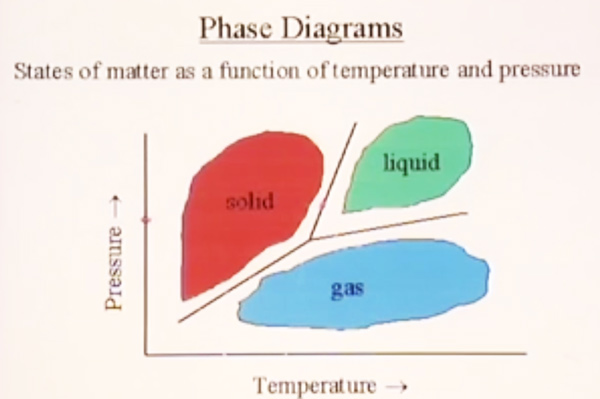
\includegraphics[scale=0.65]{Graphics/lec33_phase_diagram}
\end{center}

Consider starting at a low pressure, with the temperature at about the center, say around the ``g'' in gas. Clearly, the substance is a gas at this point. We increase the pressure,  while keeping the temperature constant. The volume decreases, and the pressure increases, with $P V$ being kept constant (which is called Boyle's law; it states that $P \propto \frac{1}{V}$ or $PV = \text{constant}$ if temperature/amount of gas is held constant). The ideal gas law holds until we reach the dividing line into the liquid. At this point, \emph{some} of the gas will turn into a liquid, and there will be an equilibrium between the two.\\
If we try to push down harder, the pressure \emph{will not increase} until \emph{all} the gas has been converted into a liquid. Only at that point will pressing harder again increase the pressure; while there is still gas present, pressing down harder will only convert more of the gas into liquid.

Suppose we instead do this at a lower temperature; we can then see that there comes a point in this example phase diagram where we go directly from gas to solid (this is called \emph{deposition}; the reverse process, solid to gas, is called \emph{sublimation}). So we increase the pressure and decrease the volume, until the solid starts forming. Once again, we can't increase the pressure further until all gas molecules are part of the solid.

Let's now look at the case of constant pressure instead of constant temperature.\\
We start out in the solid phase, at about the vertical center -- at the tiny red mark in the $y$ axis, about next to the ``e'' in pressure.\\
Say we start out with water ice; or even iron. We heat it, keeping the pressure constant, meaning we move horizontally towards the right. We eventually hit the dividing line between solid and liquid, i.e. the substance will begin to melt.\\
Once that happens, the temperature will stop increasing until \emph{all} of the solid has melted into liquid, similarly to what we saw with pressure above. Once all of it has become a liquid, we can increase the temperature further.\\
If we do so, it will eventually boil, i.e. go from a liquid to a gaseous form. Yet again, we can no longer increase the temperature at this point, until all of the liquid has become a gas (water vapor). This might be the only one of these that we are familiar with: when boiling water, it doesn't matter if the platter is just barely hot enough than necessary, or \emph{much} hotter than necessary. In either case, the liquid water will not become any hotter than 100 degrees C (unless the pressure is greater than 1 atm), no matter how violent the boiling is.

As a side note: water vapor is completely invisible (it as as transparent as clean air). Any time we think we see water vapor, for example when boiling water in the kitchen, what we actually see is tiny condensed liquid droplets. The water vapor condenses back into liquid as it comes in contact with the much colder surrounding air.\\
For this reason, you may be able to see that just above the surface of boiling water, there is invisible water vapor (i.e. it looks as if there's only air there), and only \emph{above} that is the visible steam showing up, since it hasn't had time to cool down yet when just above the surface of the boiling water.

\subsection{Pressure and phase in a CO2 fire extinguisher}

Carbon dioxide fire extinguishers are fairly common. They work by displacing oxygen, so that a fire can't be sustained. This has two important meanings, by the way: one, it can be dangerous to use on/near people or in closed spaces, as you may suffocate; two, burning materials that contain enough oxygen by themselves may well keep on burning.
 
So is there gas or liquid (or even a solid?) inside such a fire extinguisher?\\
Prof. Lewin calculated the volume of one such extinguisher to be $\SI{7.1e-3}{m^3}$. It is at room temperature, so $T = \SI{293}{K}$.

To find the pressure, which helps us find the phase, we now need to know $n$, the number of moles of CO2 inside. By reading on the label, we can find that the difference between a full extinguisher and an empty one is about 10 pounds, or 4500 grams.

Carbon has an atomic weight of about 12, and oxygen one of about 16; that gives us $A = 12 + 2\times 16 = 44$. With a molar mass of 44 g/mol, we can simply find the number of moles as

\begin{equation}
n = \frac{\SI{4500}{g}}{\SI{44}{g/mol}} = \SI{102.28}{mol} \approx \SI{100}{mol}
\end{equation}

We now have all we need to know to use the ideal gas law. We aren't sure if it will hold, but let's try. Plugging the values in,

\begin{equation}
P = \frac{n R T}{V} = \frac{ (\SI{100}{mol})(\SI{8.31}{J/(K mol)})(\SI{293}{K})}{\SI{7.1e-3}{m^3}} = \SI{3.43e7}{Pa} \approx \SI{340}{atm}
\end{equation}

This pretty much rules out the possibility of there being gas inside, for two reasons! First, it seems doubtful that the container could withstand such a tremendous pressure. Second, if we look at a phase diagram, we would likely find that CO2 becomes a liquid (or a solid) at a way lower pressure than 340 atm at room temperature. And indeed, looking at one, we find that at room temperature, the phase transition to liquid happens at something like 60-70 atm.

The answer is that the extinguisher contains a pressure of about 60 atm, according to a fire department called by the professor. Looking at a phase diagram of CO2, this makes it clear that there is either 100\% liquid, or a combination of liquid and gas inside. When we open the valve, some of the liquid will turn into gas, but the pressure will not change until all the liquid is gone. Up until that point, they must exist together, which can only happen at certain combinations of temperature and pressure. For a \emph{fixed} temperature (say 20 C), however, there is only one pressure at which this can happen; that pressure must then be constant inside until the liquid ``runs out'', having been converted into gas.

This also means we can fit a lot more CO2 into a canister than we could otherwise. Remember how the original calculations said the pressure would have to be over 300 atm if it were pure gas; with this part-liquid mix, we can fit that same amount at about 60 atm instead, which doesn't require as strong a canister. This is put to the test in a lecture question:

``The density of liquid carbon dioxide is about $\SI{0.8}{g/cm^3}$. What volume fraction inside the fire extinguisher (when it is full) is occupied by liquid CO2 ? (The density of CO2 gas is negligible compared to the density of liquid CO2)

Hint: Review what is given in the lecture: Volume of the extinguisher is $\SI{7.1e-3}{m^3}$ , total mass of CO2 = 4.5 kg, temperature= 293 K , pressure at that temperature has to be $\SI{60e5}{Pa}$.''

Hmm. Well, if 100\% was liquid, its volume would be

\begin{equation}
V = \frac{M}{\rho} = \frac{\SI{4500}{g}}{\SI{0.8}{g/cm^3}} = \SI{5625}{cm^3}
\end{equation}

... which is less than the full volume of \SI{7100}{cm^3}. In fact, it is about 80\%... a little more than 75\%, which is one of the answer options. We were told that the density of CO2 gas in negligible, so this should in fact be the answer, and it is. Not a very rigorous process, but they did tell us to neglect the gaseous portion.

\subsection{Isothermal atmosphere}

We have earlier looked at hydrostatic pressure, and found the relationship

\begin{equation}
\frac{dP}{dy} = - \rho g
\end{equation}

between pressure, density and depth. Because we can treat both $g$ and $\rho$ as constants (depth differences are small enough, and liquids are practically incompressible, respectively), this gives us a very simple linear relationship

\begin{equation}
P_2 - P_1 = -\rho g (y_2 - y_1)
\end{equation}

where $y_2 > y_1$ (positive upwards), and therefore $P_1 > P_2$. If you ever lose track of the minus signs and that, you just need to keep in mind that pressure must \emph{increase} at greater depths, and you can't go wrong. With that in mind, I probably prefer to think of this as

\begin{equation}
|\Delta P| = \rho g |\Delta y|
\end{equation}

which is hard to get wrong, using the above (rather obvious) trick.

The reason that was easy to do is that we could treat $\rho$ as constant, with little loss of accuracy. In reality, $\rho$ is a function of pressure. This is a smaller detail for liquids, but a crucial one for gases, which we'll look at now. We can no longer treat $\rho$ as a constant.

We will now look how the pressure changes in altitude in our atmosphere. We will assume that the temperature everywhere is 0 degrees C everywhere in the atmosphere; that is not true, but the full calculation is still a bit too complex. We call this simplification an isothermal atmosphere. (In general, the iso- prefix is used in physics for things that are the same in one way or another; from the Greek word isos, meaning equal.)

Density is mass per unit volume, so if we have $N$ molecules inside a certain volume $V$, each of mass $m$, we can say that

\begin{equation}
\rho = \frac{N m}{V}
\end{equation}

where $\rho$ is the average density inside that volume.

Using the ideal gas law,

\begin{align}
PV &= N k T\\
\frac{P}{k T} &= \frac{N}{V}
\end{align}

So we substitute that, and find

\begin{equation}
\rho = \frac{P m}{k T}
\end{equation}

We can then substitute that into the differential form we had earlier,

\begin{equation}
\frac{dP}{dy} = - \rho g = - \frac{P m }{k T} g
\end{equation}

Rearranged,

\begin{equation}
\frac{dP}{P}  = - \frac{m g}{k T} dy
\end{equation}

As it was before, this is a separable differential equation. $m$ is a constant, $k$ is a constant, and we said we consider $T$ and $g$ constants. The right-hand side is an easy integral, and the left-hand side isn't much harder. We integrate from $0$ (sea level) and $P_0$ to $h$ and $P_h$:

\begin{align}
\int_{P_0}^{P_h} \frac{dP}{P}  &= - \frac{m g}{k T} \int_0^h dy\\
\ln P_h - \ln P_0  &= - \frac{m g}{k T} h\\
\ln \frac{P_h}{P_0} &= - \frac{m g}{k T} h
\end{align}

Exponentiating both sides:

\begin{equation}
\frac{P_h}{P_0} = e^{- \frac{m g}{k T} h}
\end{equation}

We can still simplify this a bit. We have a constant involved; we can find its value. If we flip it upside down, the constant I'm talking about is

\begin{equation}
H_0 = \frac{k T}{m g}
\end{equation}

This is called the \emph{scale height}; it has the dimension of length, because its reciprocal (in the exponential above) must be 1 over length, so that it cancels out with $h$; you need a dimensionless number in exponentials. We know $k = R/N_A \approx \SI{1.38e-23}{J/K}$, $T = \SI{273}{K}$ (0 degrees C, as we chose earlier), and $g \approx \SI{9.8}{m/s^2}$. What about $m$, the mass of an air molecule?

Well, the professor chose to use 29 atomic mass units, with this reasoning: air is about 20\% oxygen (32 amu per molecule) and about 80\% nitrogen (28 amu per molecule), and some spare change (argon, CO2 etc) that we ignore. Since there is more nitrogen, we choose a number closer to 28 than 32 amu, and so we end up with 29 amu. (The actual value appears to be 28.964, so this approximation is very good.)\\
Each amu represents a mass of about $\SI{1.66e-27}{kg}$, so all in all, we find $H_0 \approx 8000$ meters. Rewriting our exponential, we now have

\begin{equation}
P_h = P_0 e^{- h/H_0}
\end{equation}

Using $H_0 = 8$ km and $P_0 = 1$ atm, we can then for example find that the air pressure at 3 km above sea level is about $(\SI{1}{atm})e^{-3/8}$, or about 0.7 atmospheres. At 8 km, it is only $1/e$ times 1 atm, which is about 0.37 atmospheres.

This not only has implications for human life (the air is basically too thin to support human life, though some do climb Mount Everest with no supplemental oxygen), but also for basic things like boiling water.\\
The boiling point is defined as the temperature where the liquid's \emph{vapor pressure} (which we have not really learned about in this course) equals the (atmospheric) pressure of the air surrounding the liquid.\\
The vapor pressure of a substance, e.g. water, is a constant for a given temperature. At 100 degrees, it is about 101.3 kPa (1 atm) -- that is to say, it boils at 100 degrees at 1 atmosphere. However, if the atmospheric pressure is \emph{lower}, the water will boil at a lower temperature. For example, water would boil at 80 degrees C if the atmospheric pressure were 47.3 kPa (about half an atmosphere); in other words, the vapor pressure of water is 47.3 kPa at 80 degrees C.\\
This can cause some trouble for cooking at higher altitudes -- in extreme cases, it will be hard to prepare certain types of food as they will need to boil for very long.

Even more interestingly, the vapor pressure of water at 22 degrees C is about 2.6 kPa -- which means that if we place water in a near-vacuum, it will boil at or even below room temperature. This is demonstrated in the lecture.\\
To see this on a phase diagram, locate the (likely vertical) line of constant temperature of about 20 degrees, and then find the point along that line of 1 atmosphere pressure. That's where we start out; you will undoubtedly find that the water should be in its liquid phase. Follow that line of constant temperature downwards, and you will eventually reach the line where gas and liquid coexist -- which is where it starts to boil.

\subsection{More lecture experiments}

A second lecture experiment is to add a very small amount of liquid water to a paint can (of the same type that imploded in a previous lecture, when we sucked out the air from inside it), boil it, and then seal the can. It is now filled with almost 100\% water vapor (a tiny fraction liquid water may remain), at 100 degrees C, and 1 atmosphere of pressure. We seal the can, and let it cool.

The amount of water, in moles, must of course be a constant. However, now that the temperature goes down, so does the volume of the water vapor gas; we can see this by looking at the vapor pressure for water at various temperatures. (Perhaps also by using the ideal gas law, but it doesn't hold very well for water vapor.)\\
Indeed, as it cools back down to room temperature, the vapor pressure is about 1/45 atm, so there is practically a vacuum inside (as far as the thin walls are concerned, at least), and the can will implode.

Next, we cool a regular air-filled balloon in liquid nitrogen. We change the temperature of the air inside from 293 K to about 77 K (about -196 C, the boiling point of liquid nitrogen). What will happen to the balloon?\\
We can see, using the ideal gas law, that it must shrink; if we hold $P$ approximately constant, that is clear.

\begin{align}
V_1 &= \frac{n R T_1}{P}\\
V_2 &= \frac{n R T_2}{P}\\
\frac{V_2}{V_1} &= \frac{T_2} {T_1}
\end{align}

This gives us $V_2/V_1 \approx 0.26$. The radius changes less, though; $R \propto V^{1/3}$, so the radius should shrink by something like 60\%. However, in practice, the balloon shrinks down to almost nothing -- the volume goes down to perhaps 1-2\% of the original, or something of that order.

What did we miss? Well, we used the ideal gas law -- but we won't have gases when we're done! Remember that air is 80\% nitrogen, and we dip it into liquid nitrogen. The nitrogen inside the balloon may turn into liquid, since we cool it to approximately\footnote{The heat transfer may not be ideal, etc., so it may not go all the way down to 77 K.} its boiling point.\\
The boiling point of oxygen at 1 atm is about 90.1 K, so we cool that down below its boiling point, too, so the oxygen should certainly become a liquid. We know, of course, that liquids have a \emph{way} higher density than gases, so it should not come as a huge surprise (when you consider the phase changes) that the volume is very small.



\end{document}